\documentclass[a4paper,11pt]{article}
\usepackage{graphicx,listings,a4wide,dsfont}
%\usepackage[firstpage]{draftwatermark}
%\SetWatermarkLightness{0.5}
%\SetWatermarkScale{4}
\setcounter{tocdepth}{2}

\newcommand{\question}[2]{\medskip\par\noindent\textbf{#1}\\\hangindent=0.5cm#2}

\title{Report on OGO 2.2 \\ Software specification\\ Review formal specification group 3}
\author{
        Tim van Dalen, Tony Nan, Ferry Timmers, \\ Lasse Blaauwbroek, Femke Jansen, \\Jeroen Peters and Sander Breukink\\ OGO 2.2 group 6 \\
                Department of Computer Science\\
        Technical University Eindhoven\\
}
\date{\today}

\begin{document}

\maketitle

\begin{abstract}
This document contains the review of the formal specification of group 3. We first provide some general remarks about the overall structure of the formal specification. In the sections hereafter, we provide our remarks about the Z-specification, the state diagram and the MSC's; here, we distinguish between general remarks and individual remarks about specific parts of the specification. We provide our remarks as lists, to keep them organized and readable. Finally, we give our judgement of the formal description and grade the formal description.
\end{abstract}

\newpage
	
	\tableofcontents
	\newpage
	
	\section{General remarks}
    \begin{itemize}
        \item The order of sections is not logical: the Z specification should be after the MSC's and the Statecharts.
        \item The abstract is missing.
        \item There is no content page.
        \item The introduction is short and does not tell what is coming next, so it isn't what an introduction should be like. For example, the state diagrams and MSC's are not mentioned.
        \item There are no any use case scenario's (and also no matching state diagrams and MSC's).
        \item The design decisions that have been made are not documented. For example, in our informal specification, we did not specify that player 1 always makes it turn before player 2. We would expect that you would document and motivate this decision.
        \item The class diagram is missing.
        \item It is not specified how a game ends and how the individual components of the game (Controller, Board, etc.) can conclude this and react to this.
    \end{itemize}
	
	\section{Remarks about the Z-specification}
    In this section, we organize our individual comments according to the order of the Z-schemas in the formal specification.
    \subsection{Overall remarks Z-specification}
    \begin{itemize}
        \item The description of your coordinate-system is very nice and understandable.
        \item Splitting the "MoveRequest" in Controller in several pieces was a wise decision; this way, you can keep things organized and introduce the reader step-by-step to the whole concept.
        \item Boolean is a pre-defined set in Z. The correct notation for the set of booleans is $\mathds{B}$.
        \item In sections 2 to  3.5, input-/output-variables are prefixed with a ?/!. In the remaining sections of the Z-specification, the input-/output-variables are postfixed with a ?/!. This is inconsistent and partly incorrect; input/output-variables should be postfixed with a ?/!.
        \item Some variables are unbounded or even undefined. For example, in the schema DoKill, a variable $s$ is used, but it is not clear where this variable comes from and what it's type is. The same holds for the $s?$-variable in DoMove.
        \item The MoveRequest in player checks whether is move is possible, but that is not the job of the player; the board should check whether a move request is valid.
        \item The notion of "safe tiles" is not reflected in the Z-specification. This is an important factor when a fox wants to kill a dolphin and vice versa.
        \item The notion of rounds is explained informally, but not reflected formally in the Z-specification. For example, the tides occur after completion of a round.
        \item The invariant "Two adjacent tiles (meaning they have a common edge) may only differ in two units of elevation" is not maintained in the Z-specification.
        \item You do specify a Number of Moves schema, but do not use it in MoveRequest or DoMove. A move can only be requested (and executed) if a player has any moves left.
        \item The board has a size that depends on the number of pieces. This is not reflected in the formal specification.
        \item It is not always clear where the input-, output- and dummy-variables are used for in the Z-schemas. Additional explanation would be appreciated.
    \end{itemize}

    \subsection{Pieces and players}
    \begin{itemize}
        \item One player has all pieces of type 'fox' and one player has all pieces of type 'dolphin'. You only specify that each player has pieces of the same type.
    \end{itemize}

    \subsection{Board}
    \begin{itemize}
        \item The invariant of the standard value of de height of water is bit confusing. First, you state that the x-value of a nEvent must be between -20 and 20. However, in the invariant of the standard value of the height of the water, you say that the x- and y-variables of nEvent are both natural numbers.
        \item In the informal explanation of Flood, you state that you call the Flood-function twice; however, we do not see how this is reflected in the Z-schema.
        \item In OccupiedBySameAnimal, the Z-schema is correct, but the informal explanation is not. You state the following: if the destination tile of a move request is occupied by an animal of the same type, then isOccupied is true and the move to this tile is possible. In this case, the move is, of course, not possible.
        \item In MakeMove, a conjunction is missing between the parts of the fox and the dolphin.
        \item In ShortcutPossible, both the dolphins and foxes use the bridges now as a shortcut. Dolphins should, of course, use the caves.
        \item In Init, two foxes and two dolphins should not be placed on the same tile. This is captured in MoveRequest, but it must also be captured in the initial configuration.
        \item In the informal explanation of getNrMoves, you say that the operation calculates the number of moves "automagically".
    \end{itemize}

    \subsection{Viewer and Controller}
    \begin{itemize}
        \item The initial number of foxes and dolphins can be predefined by the players. It is not clear whether this is the $n?$-variable in init; if it is, explain this in the informal description.
        \item In Init, all foxes should be placed on the land and all dolphins in the water.
    \end{itemize}

	\section{Remarks about the state diagram}
    \begin{itemize}
        \item The order of the informal explanation is inconsistent with the order of explanation in the Z-specification. In the Z-specification, you first provide the Z-schema and thereafter the explanation; in the state diagram and MSC, you first provide the explanation and thereafter the diagrams. This is inconsistent and also confusing.
        \item The state diagrams of the individual components are missing. The individual state diagrams reflect the communication within an entity (internal actions) and to the entities it "knows about"; the system state diagram is used to show how the individual entities communicate with each other.
        \item In the state diagram, it is reflected that there always is an initial flood, after the board and all its components have been initialized. There always is a flood after a round has been completed; not necessarily before the first round.
        \item A reference from a state diagram to a message sequence chart should be avoided. For every message sequence chart, there should be a state diagram which correspondents to it.
        \item All state diagrams should have a terminating state, because the game can end.
        \item A lot transition labels are incorrect. For instance, the label "MSC for P1 / End P1" of Player 1 is the part "/ End P1" not needed, since the transition "/ P2" can only be executed if state "Turn Completed" is active.
        \item There is a transition in View that does not have a label. This could either mean that it is executed immediately after the state "Updated" becomes active, or that it will be randomly executed. Explain what this transition means.
        \item Many triggers in transitions are not in the form of a method-call, like "NEvent" in Main. Explain what this label means; for example, that it is a notification that is send from one class to another
        \item The triggers of the transition in View are incorrect. According to the current state diagram, the update of the view and the update of the flood are executed concurrently, however it seems more logical that they execute sequentially.
        \item We believe a part of the following sentence is missing: "Na een beurt van een Player wordt ook het View weer up-to-date gemaakt, zoals."
    \end{itemize}
    \section{Remarks about Message Sequence Chart}
	%\subsection{Class diagram}
	The following graphic is the class diagram that will be used for the specification and the implementation. Note that, for the sake of readability, names of parameters in methods are abbreviated. For instance, the parameter 'loc' in the moveRequest of Board is in the MSCs referred to as 'localCoords', whereas in the class diagram it is abbreviated.

	%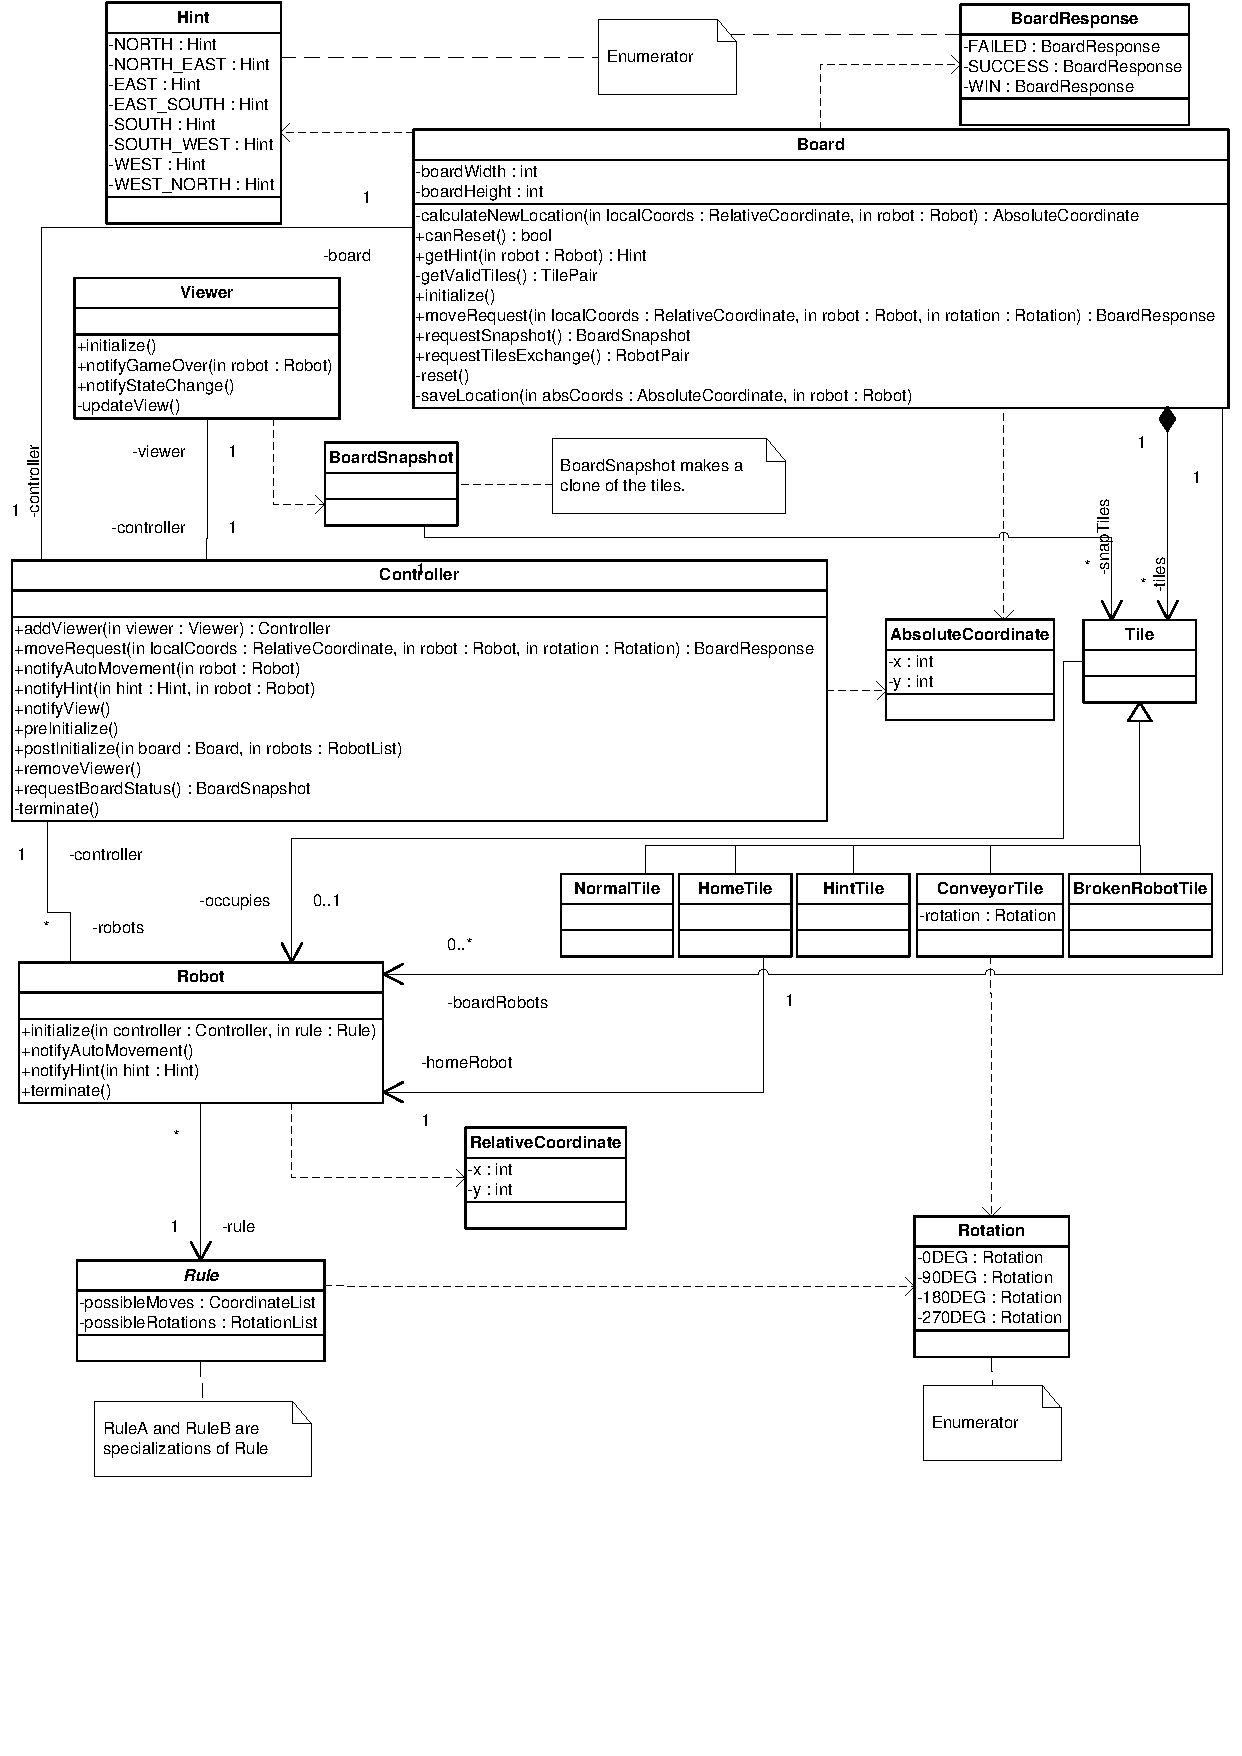
\includegraphics[width=\linewidth]{classdiagram.pdf}
	\let\l=\relax
\let\<=\relax
\let\>=\relax
\digraph[scale=.5]{classdiagram}{
margin=0
fontsize=8
fontname=Helvetica
compound=true
splines=ortho
node [fontsize=8, fontname=Helvetica, shape=record]
edge [fontsize=8, fontname=Helvetica, arrowhead=open, labeldistance=2]
Board [label="{Board|- width : int\l- height : int\l|+ canReset() : bool\l+ initialize()\l+ moveRequest(loc : RelativeCoord, r : Robot, rot : Rotation) : BoardResponse\l+ requestSnapshot() : BoardSnapshot\l+ requestTilesExchange() : bool\l- getHint(r : Robot) : Hint\l- calculateNewLocation(loc : RelativeCoord, r : Robot) :
AbsoluteCoord\l- getValidTiles() : TilePair\l- reset()\l- saveLocation(loc : AbsoluteCoord, r : Robot)\l}"]
Hint [label="{[Hint]| NORTH\l NORTH_EAST\l EAST\l SOUTH_EAST\l SOUTH\l SOUTH_WEST\l WEST\l NORTH_WEST\l}"]
BoardResponse [label="{[BoardResponse]| FAILED\l SUCCESS\l WIN\l}"]
Viewer [label="{Viewer||+ initialize()\l+ notifyGameOver(r : Robot)\l+ notifyStateChange()\l- updateView()\l}"]
BoardSnapshot [label="{BoardSnapshot||}"]
Controller [label="{Controller||+ addViewer(v : Viewer) : Controller\l+ moveRequest(loc : RelativeCoord, r : Robot, rot : Rotation) : BoardResponse\l+ notifyAutoMovement(r : Robot)\l+ notifyHint(h : Hint, r : Robot)\l+ notifyView()\l+ preInitialize()\l+ postInitialize(b : Board, rs : RobotList)\l+ removeViewer()\l+ requestBoardSnapshot() : BoardSnapshot\l- terminate()\l}"]
AbsoluteCoord [label="{AbsoluteCoord|+ x : int\l+ y : int\l|}"]
Tile [label="{Tile||}"]
/**/
subgraph cluster_Tiles {
NormalTile [label="{NormalTile||}"]
HomeTile [label="{HomeTile||}"]
HintTile [label="{HintTile||}"]
ConveyorTile [label="{ConveyorTile|- rot : Rotation|}"]
BrokenRobotTile [label="{BrokenRobotTile||}"]
}
/**/
Robot [label="{Robot||+ initialize(c : Controller, r : Rule)\l+ notifyAutoMovement()\l+ notifyHint(h : Hint)\l+ terminate()\l}"]
RelativeCoord [label="{RelativeCoord|+ x : int\l+ y : int\l|}"]
Rule [label="{\<\<Rule\>\>|- possibleMoves : RelativeCoordList\l- possibleRotations : RotataionList\l|}"]
Rotation [label="{[Rotation]| 0DEG\l 90DEG\l 180DEG\l 270DEG\l}"]
/**/
Board->Controller [taillabel=1, headlabel="0..*"]
Board->Tile [arrowtail=diamond,dir=both, taillabel=1,headlabel="*"]
Board->Robot [taillabel=1, headlabel="0..*"]
/**/
Controller->Viewer [taillabel=1, headlabel=1, arrowhead=none]
Controller->Robot [taillabel=1, headlabel="*", arrowhead=none]
/**/
Tile->Robot [taillabel=1, headlabel="              0..1 - occupier"]
/**/
HomeTile->Robot [taillabel=1, headlabel="              1 - homeRobot"]
/**/
Robot->Rule [taillabel="*", headlabel=1]
/**/
BoardSnapshot->Tile [taillabel=1, headlabel="*"]
/**/
NormalTile->Tile [ltail=cluster_Tiles,arrowhead=empty]
/**/
Board->Hint [style=dashed]
Board->BoardResponse [style=dashed]
Board->AbsoluteCoord [style=dashed]
Viewer->BoardSnapshot [style=dashed]
Controller->AbsoluteCoord [style=dashed]
Robot->RelativeCoord [style=dashed]
Rule->Rotation [style=dashed]
ConveyorTile->Rotation [style=dashed]
} 
    Abstract classes are indicated by guillemets and enumerators by brackets.

\subsection{Class description}
    Next, a description will be given about all the classes in the class diagram. Here, the function of the class can be found, along with its attributes and its functions (and description of these). Since some of the functions have a lot of arguments, these arguments are not showed here. Note that most relations in the class diagram are undirected; for example, the robot has no knowledge about the board, so the association between Board and Robot is directed. The controller and the viewer, however, do have knowledge about each other, so this is an undirected association.

	\begin{description}
        \item[Hint] An enumeration that contains all possible hints that a Robot can receive from a hint tile.
        \item[BoardResponse] An enumerator that contains all the possible responses that the board can give the controller when it makes a move request.
		\item[Board] This class contains the functionality of the board. It contains the following attributes:
        \begin{description}
            \item width: The private variable which contains the width of the board.
            \item height: The private variable which contains the height of the board.
        \end{description}
        Furthermore, the following functions are present:
        \begin{description}
            \item canReset(): The public method which checks if the board can reset. The board can reset if a robot has reached its home tile and a new game can begin.
            \item initialize(): The public method to initialize the board (and with this, also the controller and the robots).
            \item moveRequest(): The public method which handles move requests forwarded by the controller. This method first checks if the move is valid (otherwise, return the BoardResponse FAILED), next it calls calculateNewLocation() to calculate the new location of the robot. After that, saveLocation is called to save the location and the proper board response is returned. Sometimes the board also sends a hint or a notification of an automovement.
            \item requestTilesExchange(): This public method handles with the tiles exchange after a robot has made his move. First it calls getValidTiles() to make sure that the invariant still holds after the exchange. Next it swaps the tiles and handles possible robot replacements or movements.
            \item getHint(): This private method gets an appropriate hint for the robot.
            \item calculateNewLocation(): This private method (used in moveRequest()) calculates the new location of a robot, according to his current position and the position he wants to move to. It also deals with conveyor tiles and broken robot tiles.
            \item getValidTiles(): This private method is used to get two tiles that can be switched, hereby not violating the invariant.
            \item reset(): This private method is used to reset the board. canReset() should return true in order for this function to be called. The board then makes the other components terminate and can initiate new components (e.g. controller, robots) in order to start a new game.
            \item saveLocation(): This private method is used to save the new location of a robot; it is called in moveRequest().
        \end{description}
		\item[Controller] This class represents the controller, which is used as mostly used as communication device between the board and other components. The controller has a viewer, as shown on the undirected association between Controller and Viewer. The controller has the following functions:
        \begin{description}
            \item addViewer(): This public method is used to add a viewer to the controller, so that the controller can notify this viewer when there is a change in the board (see the association in the class diagram).
            \item moveRequest(): This public method is used to forward move requests from the robot. The robot calls this function and the controller calls the moveRequest() function from the board with the right parameters.
            \item notifyAutoMovement(): This public method is used to notify the robot that is has been moved without the robot wanting to; for example, because of a conveyor tile or a tiles exchange.
            \item notifyHint(): This public method is used to notify a robot that it is on a hint tile and what direction he has to go in order to find his home tile.
            \item notifyViewer(): This public method is used to notify the viewer that the board has changed. A snapshot will be send to the viewer.
            \item preInitialize(): This public method is used to pre-initialize the controller, so that there exists an object of the type controller.
            \item postInitialize(): This public method is used to (after pre-initialization) fully initialize the controller with a board and the robots.
            \item removeViewer(): This public method is used to remove a viewer from the controller. This function can be used to add a new viewer or before termination.
            \item terminate(): This function is used to first terminate all objects (except for board). After these objects have been terminated, it informs the board about this; afterwards, the controller itself terminates.
        \end{description}
        \item[Viewer] This class describes the functionality of the viewer, so that the game can be watched. This class has no special attributes. It contains the following functions:
        \begin{description}
            \item initialize(): This public method is used to initialize a viewer.
            \item notifyGameOver(): This public method is used to notify the viewer that a robot has reached its home tile. Fireworks will be shown and after this the viewer can terminate.
            \item notifyStateChange(): This public method is used to notify the viewer that the board has changed, hereby receiving a new snapshot of the board. After this, updateView() will be called to deal with the new snapshot.
            \item updateView(): This private method deals with new snapshots of the board and makes sure that they will be shown.
        \end{description}
        \item[AbsoluteCoord] A data class that contains the x and y coordinate of an absolute coordinate.
		\item[BoardSnapshot] A data class that contains a snapshot of the board, i.e. a copy of all the tiles in the board.
		\item[Tile] Used to model the tiles that the Board consists of.
		\item[NormalTile] Tiles without a special meaning (specialization of the Tile class).
		\item[HomeTile] Tiles that are the "home" of a robot (specialization of the Tile class).
		\item[HintTile] Tiles that return a hint as to where the robot's home is (specialization of the Tile class).
		\item[ConveyorTile] Tiles that change the position and rotation of robots (specialization of the Tile class).
		\item[BrokenRobotTile] Tiles that are occupied by a defective robot (specialization of the Tile class).
		\item[Robot] This class is used for the functionality of robots, both of type A or B in the informal specification. This class has a rule, as shown on the directed association between Robot and Rule. This class has the following functions:
        \begin{description}
            \item initialize(): This public method is used to initialize a given robot, hereby also initializing its rule, a robot of type A or B will then start.
            \item notifyAutomovement(): This public method is used to notify the robot that it has been moved automatically (e.g. by a conveyor tile or by the tiles exchange).
            \item notifyHint(): This public method is used to notify a robot that it has stepped on a hint tile and what direction he has to go in order to find his home tile.
            \item terminate(): This public method is used to make the robot terminate.
        \end{description}
		\item[Rule] An abstract class that is used to model the behaviour of Robot A and B in the Robot class. Any class that defines a rule inherits from this class. This class does not contain any functions. This class has the following attributes:
        \begin{description}
            \item possibleMoves: A list of relative coordinates where the robot is allowed to move to.
            \item possibleRotations: A list of rotations the robot is allowed to do.
        \end{description}
		\item[RelativeCoord] A data class that contains the x and y coordinate of a relative coordinate.
		\item[Rotation] An enumeration that is used to model the rotation in robots and conveyors.
	\end{description}

    \begin{itemize}
        \item In the MSC is shown that a round begins with a call from the controller to the board, to request the number of moves of a player. We did not state this in our informal specification. A player first makes a move request, the controller then forwards this request to the board. Since the board knows the number of moves for each player, it can internally determine whether a move request is valid, based upon these number of moves.
        \item The "request move"-message from controller to player should go the other way around. As explained above, the player requests a move; the controller does not ask the player whether it wants to move.
    \end{itemize}

    \section{Judgement and grading}
    \subsection{Consistency}
    ToDo

    \subsection{Correspondence to the informal description}
    ToDo

    \subsection{Completeness}
    ToDo

    \subsection{Explanation and coherence}
    ToDo
\end{document} 